\section{Example}
\label{subsec:example}
%Step-by-step example (intention is to move this to an appendix)
Here, a contrived Hamiltonian is used to show the step-by-step procedure of LOBE. The example Hamiltonian, with a bosonic occupancy cutoff $\Omega = 3$, that will be used is 

\begin{equation}
    \label{eq:example-ham}
    H = b_0^\dagger d_0(a_0^\dagger)^2 + 2 d_0^\dagger a_0^\dagger a_0+3 b_0^\dagger d_0^\dagger d_0
\end{equation}

\textbf{Step 1: Rescale Hamiltonian from bosonic terms:}
To rescale the coefficients of the Hamiltonian due to the presence of bosonic operators, equation \ref{bose coeff rescale}, is used. If we let $\alpha_0 = 1, \alpha_1 = 2, \alpha_2 = 3$, we obtain  $\alpha_0^* = 1,\alpha_1^* = 2, \alpha_2^* = 0.75$ since $K = 2$. Thus,
\begin{equation}
    \tilde{H} = b_0^\dagger d_0(a_0^\dagger)^2 + 2 d_0^\dagger a_0^\dagger a_0+0.75 b_0^\dagger d_0^\dagger d_0
\end{equation}

\textbf{Step 2: Rescale coefficients of Hamiltonian:} In order to load the Hamiltonian coefficients into the circuit via the $R_y$ gates in the \textit{coefficient} oracle, we need to ensure the coefficients are $\leq 1$. This procedure is done differently for \textit{USP} and \textit{ASP}. The goal is to get $H^* = \frac{\tilde{H}}{\lambda}$, where $\lambda$ is different depending on the state preparation routine.
\begin{enumerate}
    \item \textbf{USP}: The \textit{prepare} oracle with \textit{USP} is done by dividing each coefficient of $\tilde{H}$ by the maximum coefficient, $\max{|\tilde{\alpha}_l|}$. Thus, the $R_y$-\textit{gate} coefficients are $\frac{1}{2}, 1, \frac{3}{8}$ respectively. To get the total rescaling factor of the Hamiltonian, equation \ref{usp scale} is used. In this case, $L = 3$ since there are three terms, and $\alpha^* = 2$, the largest term coefficient of $\tilde{H}$. Thus, $\lambda_{usp} = 2^{\lceil \log_2{3} \rceil}\alpha^* = 8$. 
    \item \textbf{ASP}: The \textit{prepare} oracle with \textit{ASP} is done by rescaling the coefficients of $\tilde{H}$ by their \textit{L1 - norm} \ref{eq:asp-scale}. Thus, $\lambda_{asp} = |1| + |2| + |0.75| = 3.75$.
\end{enumerate}

\textbf{Step 3: Obtain the corresponding LOBE circuit:} In the style of figure \ref{fig:select-normal-ordering}, for this particular Hamiltonian, the three \textit{select} oracle unitaries: $U_{T_0}, U_{T_1}, U_{T_2}$ appear as:
\begin{figure}[h]
    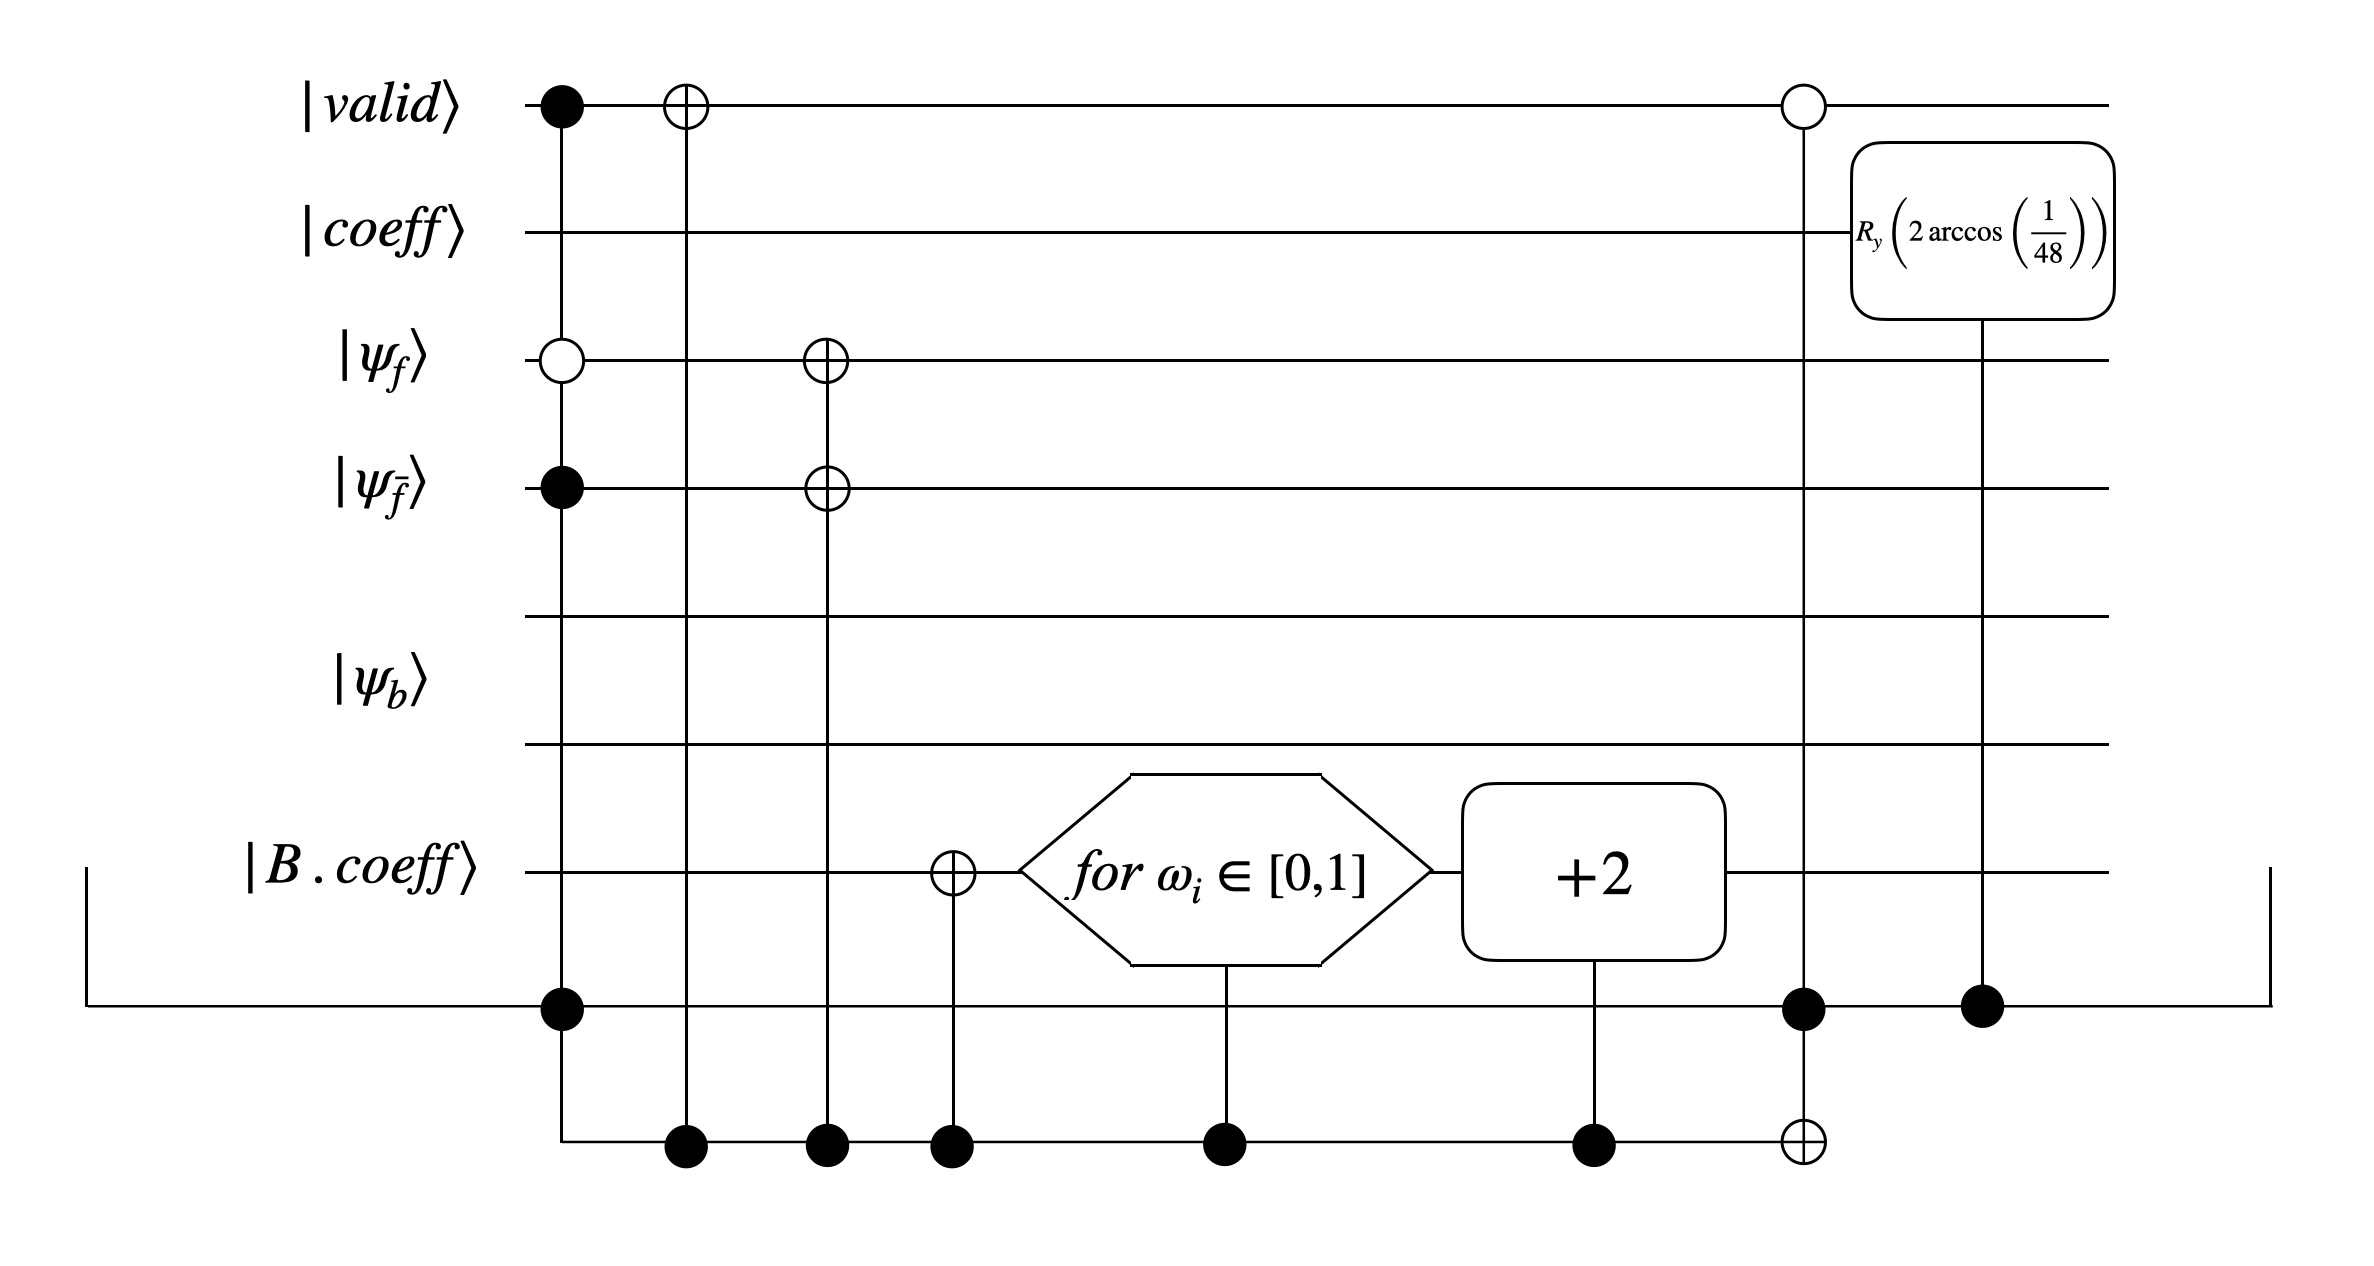
\includegraphics[width = 0.7\linewidth]{figures/T0.png}
    \caption{\textit{Select} unitary $U_{T_0}$ that block-encodes $T_0 = \frac{1}{2}b_0^\dagger d_0(a_0^\dagger)^2$}
\end{figure}
\begin{figure}[h]
    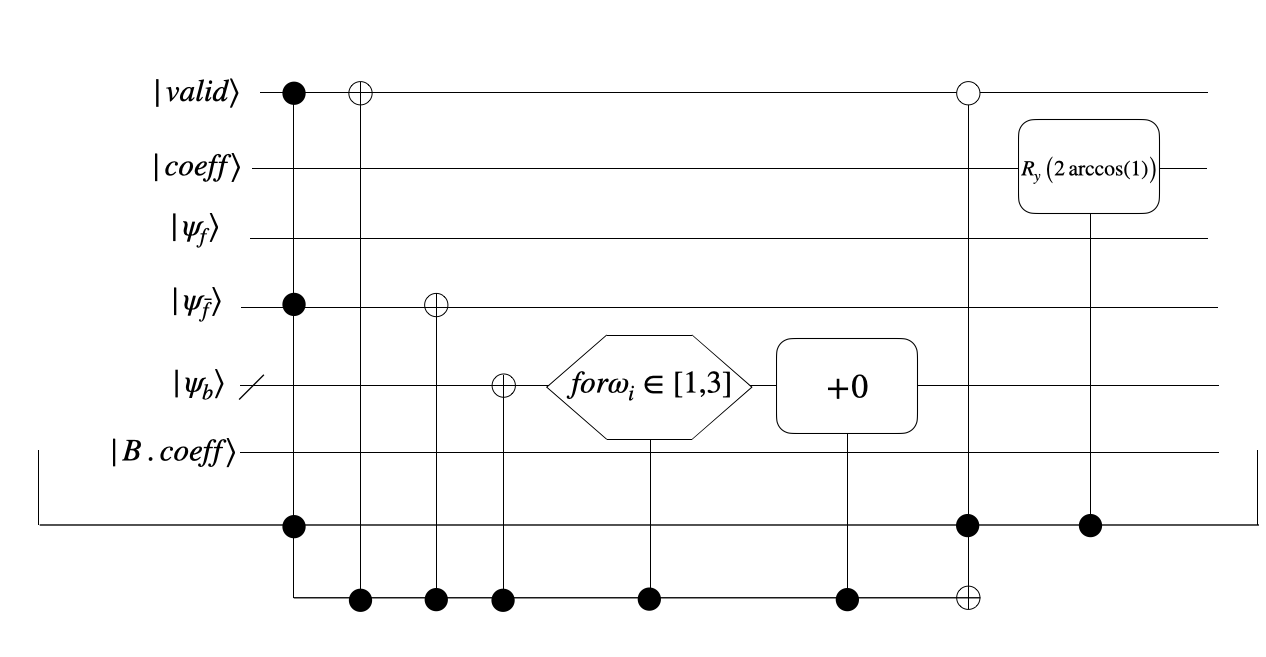
\includegraphics[width = 0.7\linewidth]{figures/T1.png}
    \caption{\textit{Select} unitary $U_{T_1}$ that block-encodes $T_1 = d_0^\dagger a_0^\dagger a_0 $}
\end{figure}
\begin{figure}[h]
    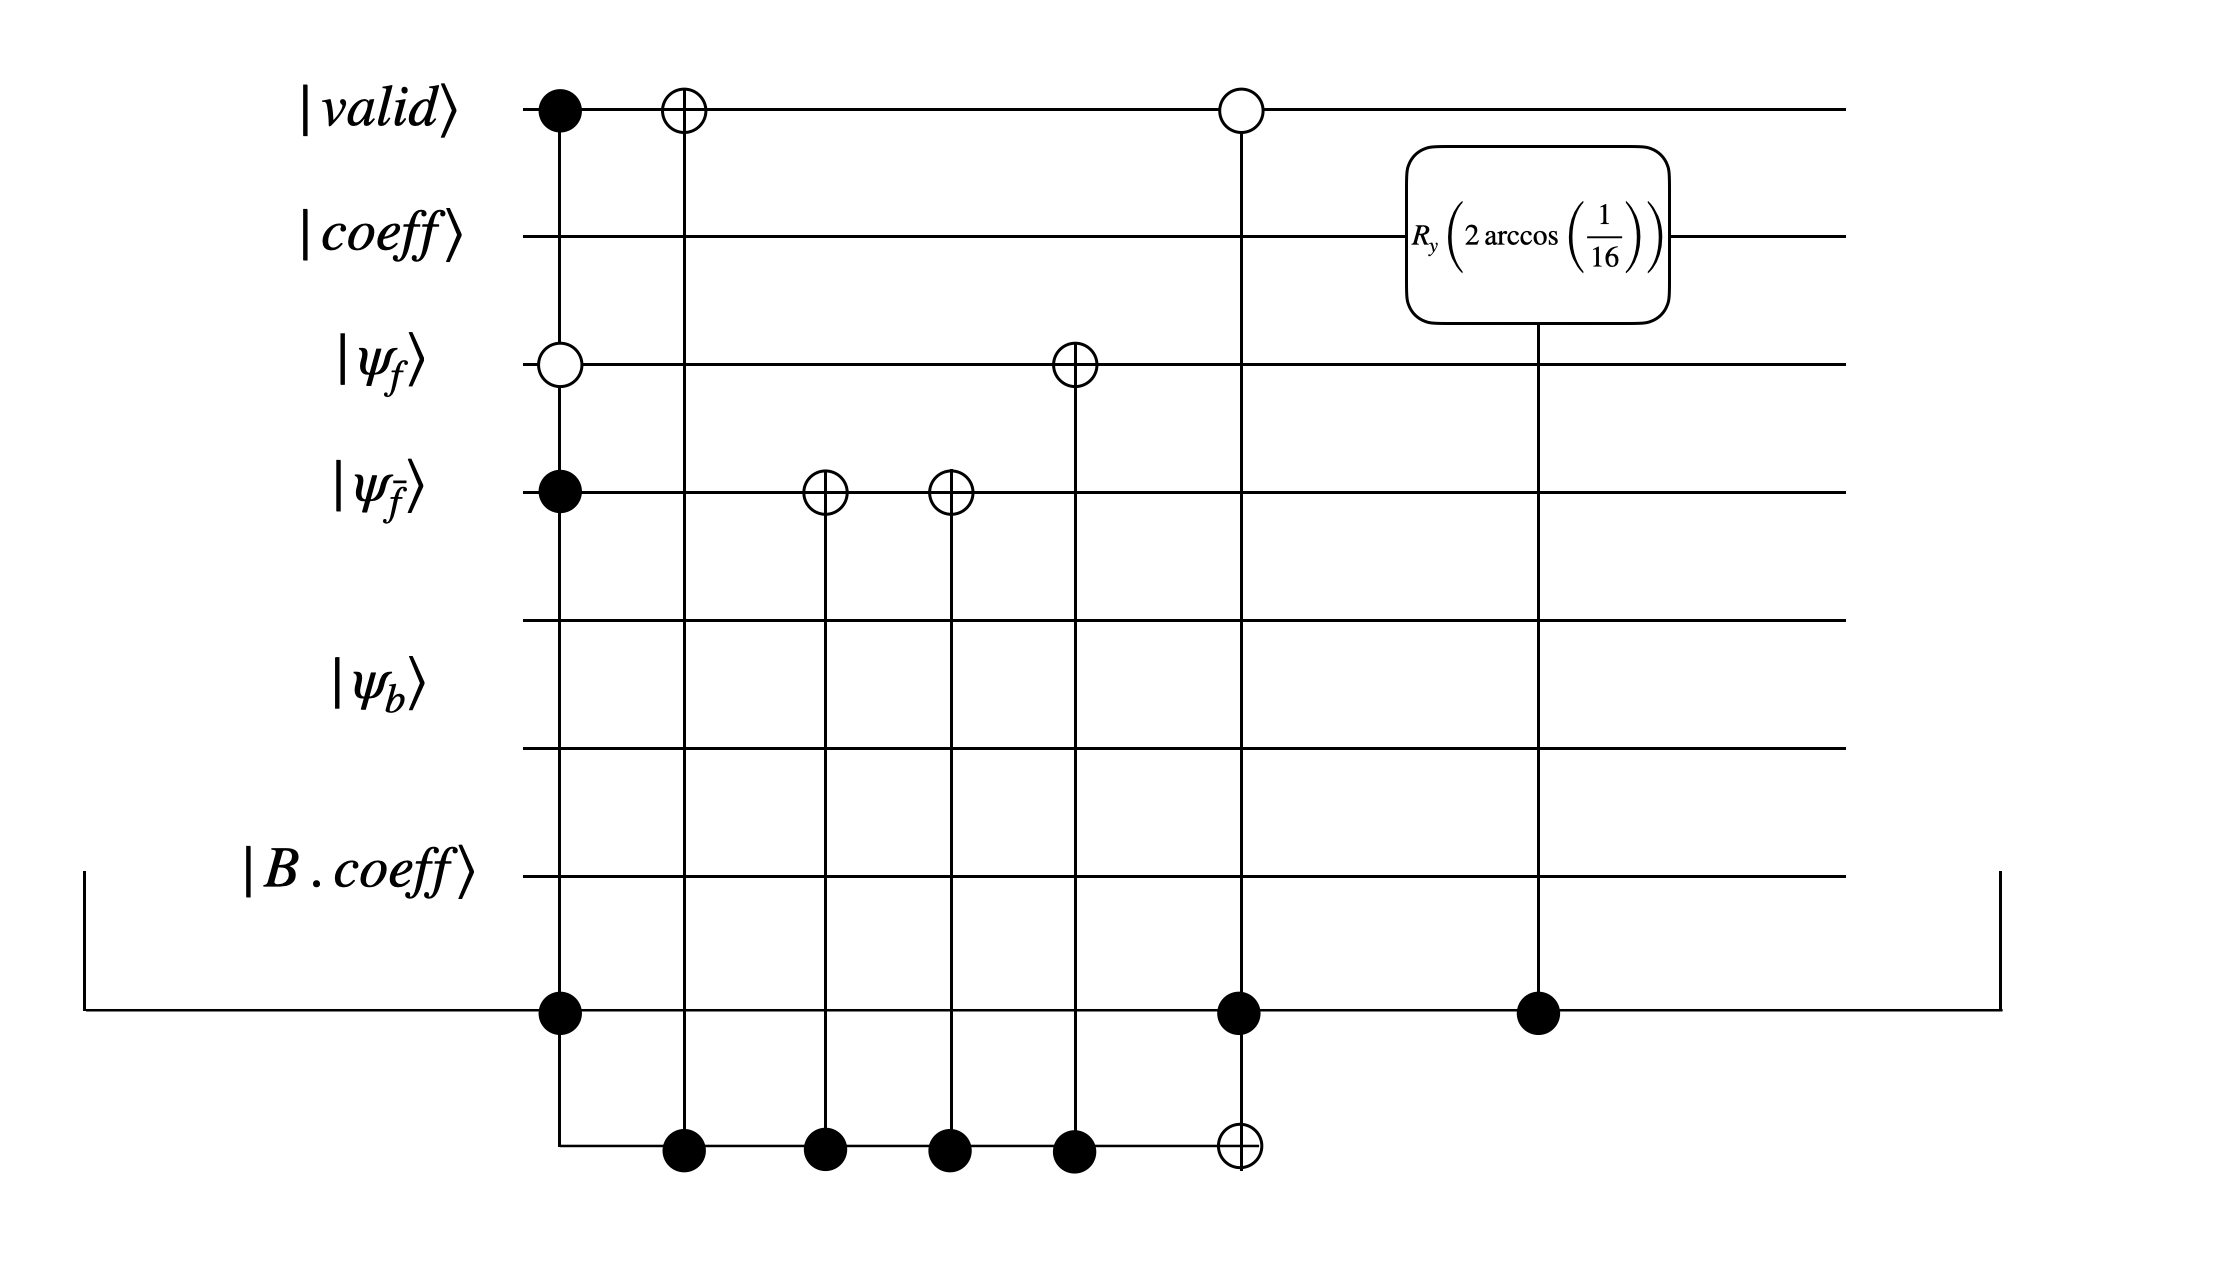
\includegraphics[width = 0.7\linewidth]{figures/T2.png}
    \caption{\textit{Select} unitary $U_{T_2}$ that block-encodes $T_2 = \frac{3}{16}b_0^\dagger d_0^\dagger d_0$}
\end{figure}

\textbf{Step 4: Count gates:} Using the notation in \ref{count gates not.}, the preceeding three unitaries have the following gate counts:

\begin{center}
    \begin{tabular}{ |p{2cm}||p{3cm}|p{3cm}|}
        \hline
        $C$& USP &ASP\\
        \hline
        $U_{T_0}$   & $(8, 8, 7)$    &$(6, 8, 7)$\\
        $U_{T_0}$   & $(8, 7, 6)$    &$(6, 7, 6)$\\
        $U_{T_0}$   & $(2, 4, 3)$    &$(0, 4, 3)$\\
        \hline
        $C_{\text{SELECT}}$ & $(18, 21, 18)$ &$(12, 21, 18)$\\
        $C_{\text{PREPARE}}$ & $(0, 0, 0)$ &$(3, 0, 0)$\\
        \hline
        $C_{\text{Total}}$ & $(18, 21, 18)$& $(18, 21, 18)$\\
        \hline
       \end{tabular}
\end{center}

Note that the counts for $C_{\text{SELECT}}$ are not simply the sum of the cost of the unitaries above because when we add in the cost of the controlled multiplexor over the index register, we add two more left and right elbows ($N_{elbows} = L - 1$, where $L$ is the number of terms). 

\textbf{Step 5: Post-process the eigenvalues:} After obtaining the full block-encoding of the Hamiltonian, the eigenvalues (which can be obtained via phase estimation) must be post-processed. This is because the eigenvalues of the block encoded Hamiltonian will correspond to $H^*$, \textit{not} $H$ (the original problem Hamiltonian).
The final scaling of the Hamiltonian that needs to be post-processed is given in equation \ref{eq:post-process}. $(\Omega + 1)^{K / 2}$ is the same for \textit{USP} and \textit{ASP}; however, the additional scaling factor $\lambda$ will change $H^*$, depending on the preparation protocol. It is easy to calculate $(\Omega + 1)^{K/2} = 4^{2/2}$, and we obtained $\lambda_{usp} = 8$ and $\lambda_{asp} = 3.75$ in step 3. 
We then can get $H^*_{\text{USP}} = \frac{H}{32}$, and $H^*_{\text{ASP}} = \frac{H}{15}$. Thus, $E_{USP} = 32E^*_{USP}$ and $E_{ASP} = 15E^*_{ASP}$.